\documentclass[margin=0mm,tikz]{standalone}

\usepackage{tikz}
\usepackage{xcolor}

\usetikzlibrary{positioning}
\usetikzlibrary{fit}
\usetikzlibrary{calc}
\usetikzlibrary{arrows.meta}
\usetikzlibrary{quotes}
\usetikzlibrary{backgrounds}

\pgfdeclarelayer{background}
\pgfsetlayers{background,main}

% -----------------------
% colors
% -----------------------
\definecolor{polar1}{RGB}{180, 203, 231}
\definecolor{polar2}{RGB}{172, 192, 231}
\definecolor{equat1}{RGB}{231, 213, 168}
\definecolor{equat2}{RGB}{231, 203, 173}


% Set background color
%\pagecolor{white}


\tikzstyle{p1face} = [
	draw=polar1,
	top color=polar1,
	bottom color=polar1,
	minimum size=1.5cm,
	rotate=-45
]
\tikzstyle{p2face} = [
	draw=polar2,
	top color = polar2,
	bottom color = polar2,
	minimum size=1.5cm,
	rotate=-45
]
\tikzstyle{e1face} = [
	draw=equat1,
	top color = equat1,
	bottom color = equat1,
	minimum size=1.5cm,
	rotate=-45
]
\tikzstyle{e2face} = [
	draw=equat2,
	top color = equat2,
	bottom color = equat2,
	minimum size=1.5cm,
	rotate=-45
]


\begin{document}
	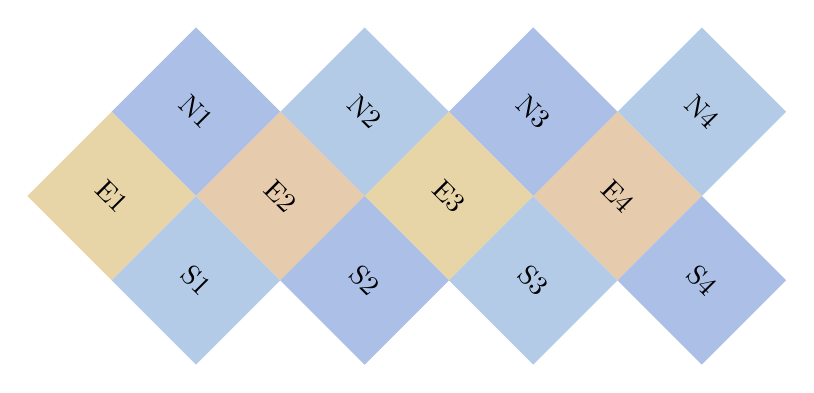
\begin{tikzpicture}[node distance=0.0cm and 0.0cm]
	
	%
	% Ordering of all faces
	
	% North faces
	\node[p2face] (N1) {N1};
	\node[p1face, above right=of N1] (N2) {N2};
	\node[p2face, above right=of N2] (N3) {N3};
	\node[p1face, above right=of N3] (N4) {N4};
	
	% Equator faces
	\node[e1face, below=of N1] (E1) {E1};
	\node[e2face, below=of N2] (E2) {E2};
	\node[e1face, below=of N3] (E3) {E3};
	\node[e2face, below=of N4] (E4) {E4};
	
	% Equator faces
	\node[p1face, right=of E1] (S1) {S1};
	\node[p2face, right=of E2] (S2) {S2};
	\node[p1face, right=of E3] (S3) {S3};
	\node[p2face, right=of E4] (S4) {S4};
		
	\end{tikzpicture}
\end{document}